\documentclass[17pt]{beamer}
\usepackage[utf8]{inputenc}
\usepackage{bookman} %font style
\usepackage{multicol}
\usepackage{cancel}
\usepackage{tikz}
\usepackage{xcolor} % for font color
\usetikzlibrary{calc}
\usetikzlibrary{positioning}
\usetikzlibrary{arrows.meta}
\usetikzlibrary{angles,quotes}
%\usetikzlibrary{decorations.pathreplacing}
\usepackage{wasysym} %for checked symbol 
\usepackage{tabularx} 
\usepackage{color, colortbl} %coloring table cells
\usepackage{gensymb} %degree symbol
\usepackage{amsfonts} %integer symbol
\usepackage{pgfplots} %graphs
\usepackage{easytable} % TAB
\usepackage{siunitx} % celsius symbol
\usepackage{stackengine} %to define \pesos 
\usepackage{systeme} % system of equations
\usepackage{pifont} % cross mark

\newcommand\pesos{\stackengine{-1.1ex}{P}{\stackengine{-1ex}{$-$}{$-$}{O}{c}{F}{F}{S}}{O}{c}{F}{T}{S}} 

\definecolor{Lgray}{gray}{0.9}
\definecolor{Dgray}{gray}{0.6}

\newcolumntype{Y}{>{\centering\arraybackslash}X} %for tabularx

\makeatletter
\newlength\beamerleftmargin
\setlength\beamerleftmargin{\Gm@lmargin}
\makeatother

\newcommand{\void}{\text{\hspace{2em}}}

\newcommand{\minivoid}{\text{\hspace{1em}}}

\newcommand{\sol}[3]{\begin{tikzpicture}[remember picture, overlay]
		\color{red}
        \node at (current page.south west) (sw) {};
		\node[anchor=south west, inner sep=0pt] at ($(sw) + (#1, #2) $)   (a) {
			\begin{minipage}[t]{0.75\textwidth}
				#3
			\end{minipage}};
    \end{tikzpicture}}


\newcommand \redcheck {{\color{red}\checkmark}}

\newcommand \redcross {{\color{red}\ding{56}}}

\newcommand{\vone}{\vspace{1em}}

\newcommand{\vhalf}{\vspace{0.5em}}

\newcommand{\mygrid}[2]{\begin{center}
		\begin{tikzpicture}[scale=#1]		
			\draw [help lines] (-10, -10) grid (10, 10);
			\draw[line width=0.5mm, <->, >={Latex[round]}] (-10, 0) -- (10, 0);
			\draw[line width=0.5mm, <->, >={Latex[round]}] (0, -10) -- (0, 10);	
			\input{#2}
		\end{tikzpicture}  
	\end{center}} 

\newcommand{\arrowcomment}[9]{\begin{tikzpicture}[remember picture, overlay]
		\node at (current page.south west) (sw) {};
		\node[anchor=south west, inner sep=0pt] at ($(sw) + (0, 0) $)   (a) {
			\begin{tikzpicture}[->,>=stealth, thick, main node/.style={rectangle,font=\sffamily\bfseries}, remember picture, overlay]

				\node (1)  at (#1, #2) {};

				\node[main node] (2)  at (#3, #4) {#5};

				\draw [->, red] (1.#6) to [out=#8,in=#9] (2.#7);

			\end{tikzpicture}
		};
\end{tikzpicture}} 

\newcommand{\plotit}[3]{\begin{center}
		\begin{tikzpicture}[scale=#2, main node/.style={rectangle,font=\sffamily\bfseries}]		
			\draw [help lines] (-#3, -#3) grid (#3, #3);
			\draw[line width=0.5mm, <->, >={Latex[round]}] (-#3, 0) -- (#3, 0);
			\draw[line width=0.5mm, <->, >={Latex[round]}] (0, -#3) -- (0, #3);	
			\input{#1}
		\end{tikzpicture}  
\end{center}} 

\newcommand{\plotpoint}[7]{\begin{center}
		\begin{tikzpicture}[scale=#7]		
			\coordinate (a) at (#1, #2);
			\draw [help lines] (-#5, -#5) grid (#5, #5);
			\draw[line width=#6 mm, <->, >={Latex[round]}] (-#5, 0) -- (#5, 0);
			\draw[line width=#6 mm, <->, >={Latex[round]}] (0, -#5) -- (0, #5);	
			\fill [fill=black] (a) circle (#3 pt);
			\node[anchor=#4, inner sep=2pt, rotate=0] (a-label) at (a) {$(#1, #2)$};
			\end{tikzpicture}  
	\end{center}} 

\newcommand{\plotoverlay}[5]{\begin{tikzpicture}[remember picture, overlay]
		\node at (current page.south west) (sw) {};
		\node[anchor=south west, inner sep=0pt] at ($(sw) + (#1, #2) $)   (a) {
			\begin{minipage}[t]{0.75\textwidth}
				 \begin{tikzpicture}[scale=#4, remember picture, overlay]		

						\draw [help lines] (-#5, -#5) grid (#5, #5);

						\draw[line width=0.5mm, <->, >={Latex[round]}] (-#5, 0) -- (#5, 0);

						\draw[line width=0.5mm, <->, >={Latex[round]}] (0, -#5) -- (0, #5);	

						\input{#3}

				\end{tikzpicture}
		\end{minipage}};
\end{tikzpicture}}

\newcommand{\lcmthreebythree}[9]{\begin{tikzpicture}[remember picture, overlay]
		\color{red}
		\node at (current page.south west) (sw) {};
		\node[anchor=south west, inner sep=0pt] at ($(sw) + (#1, #2) $)   (a) {
			\begin{minipage}[t]{0.75\textwidth}
				\pause Find the LCM: \\

				\begin{tabular}{rclll}

					$ \pause #3 $ & $=$ & $ \pause #6 $ & & \\

					$ \pause #4 $ & $=$ &  & $ \pause #7$ & \\

					$ \pause #5  $ & $=$ &  & & $ \pause #8 $ \\

					\hline

					\pause LCM & $=$ & \pause $ (#6) $ & \pause $ (#7) $ & \pause $ (#8) \pause = #9 $  \\

				\end{tabular}
		\end{minipage}};
\end{tikzpicture}}


\newcommand{\lcmtwobytwolineone}[3]{
	\def \lcmtwobytwolineonenumber {#1}
	\def \lcmtwobytwolineonefactorone {#2}
	\def \lcmtwobytwolineonefactortwo {#3}}

\newcommand{\lcmtwobytwolinetwo}[3]{
	\def \lcmtwobytwolinetwonumber {#1}
	\def \lcmtwobytwolinetwofactorone {#2}
	\def \lcmtwobytwolinetwofactortwo {#3}
%	\lcmtwobytwolineone
}

\newcommand{\lcmtwobytwolinethree}[3]{
	\def \lcmtwobytwolinethreelcm {#3}
	\def \lcmtwobytwolinethreefactorone {#1}
	\def \lcmtwobytwolinethreefactortwo {#2}
%	\lcmtwobytwolinetwo
}

\newcommand{\lcmtwobytwo}[2]{\begin{tikzpicture}[remember picture, overlay]
%		\lcmtwobytwolinethree
		\color{red}
		\node at (current page.south west) (sw) {};
		\node[anchor=south west, inner sep=0pt] at ($(sw) + (#1, #2) $)   (a) {
			\begin{minipage}[t]{0.75\textwidth}
				\pause Find the LCM: 
				
				\begin{tabular}{rccccc}

					$ \pause \lcmtwobytwolineonenumber $ & $=$ & $ \pause \lcmtwobytwolineonefactorone $ & $ \pause \lcmtwobytwolineonefactortwo $ & & \\

					$ \pause \lcmtwobytwolinetwonumber $ & $=$ & $ \pause \lcmtwobytwolinetwofactorone $ & $ \pause \lcmtwobytwolinetwofactortwo $ & & \\

					\hline

					\pause LCM & $=$ & \pause $ (\lcmtwobytwolinethreefactorone) $ & \pause $ (\lcmtwobytwolinethreefactortwo) $ & $=$ & \pause $ \lcmtwobytwolinethreelcm $  \\

				\end{tabular}
		\end{minipage}};
\end{tikzpicture}}


\newcommand{\lcmtwobythreelineone}[4]{
	\def \lcmtwobythreelineonenumber {#1}
	\def \lcmtwobythreelineonefactorone {#2}
	\def \lcmtwobythreelineonefactortwo {#3}
	\def \lcmtwobythreelineonefactorthree {#4}}

\newcommand{\lcmtwobythreelinetwo}[4]{
	\def \lcmtwobythreelinetwonumber {#1}
	\def \lcmtwobythreelinetwofactorone {#2}
	\def \lcmtwobythreelinetwofactortwo {#3}
	\def \lcmtwobythreelinetwofactorthree {#4}
}

\newcommand{\lcmtwobythreelinethree}[4]{
	\def \lcmtwobythreelinethreefactorone {#1}
	\def \lcmtwobythreelinethreefactortwo {#2}
	\def \lcmtwobythreelinethreefactorthree {#3}
	\def \lcmtwobythreelinethreelcm {#4}
}

\newcommand{\lcmtwobythree}[2]{\begin{tikzpicture}[remember picture, overlay]
		\color{red}
		\node at (current page.south west) (sw) {};
		\node[anchor=south west, inner sep=0pt] at ($(sw) + (#1, #2) $)   (a) {
			\begin{minipage}[t]{0.75\textwidth}
				\pause Find the LCM: 
				
				\begin{tabular}{rcccccc}
					
					$ \pause \lcmtwobythreelineonenumber $ & $=$ & $ \pause \lcmtwobythreelineonefactorone $ & $ \pause \lcmtwobythreelineonefactortwo $ & $ \pause \lcmtwobythreelineonefactorthree $ & & \\
					
					$ \pause \lcmtwobythreelinetwonumber $ & $=$ & $ \pause \lcmtwobythreelinetwofactorone $ & $ \pause \lcmtwobythreelinetwofactortwo $ & $ \pause \lcmtwobythreelinetwofactorthree $ & & \\
					
					\hline
					
					\pause LCM & $=$ & \pause $ (\lcmtwobythreelinethreefactorone) $ & \pause $ (\lcmtwobythreelinethreefactortwo) $ & \pause $ (\lcmtwobythreelinethreefactorthree) $ & $=$ & \pause $ \lcmtwobythreelinethreelcm $  \\
					
				\end{tabular}
		\end{minipage}};
\end{tikzpicture}}

\newcommand{\plotsystvars}[8]{
	\def \eqone {#1}
	\def \eqtwo {#2}
	\def \solx {#3}
	\def \soly {#4}
	\def \solanchor {#5}
	\def \labelxshift {#6}
	\def \labelyshift {#7}
	\def \solmarksize {#8}
}

\newcommand{\plotsyst}[7]{
\begin{tikzpicture}[scale=#1]
	
	\begin{axis} 
		[
		xticklabels={}, 
		yticklabels={}, 
		ymin=-#2, ymax=#2,
		xmin=-#2, xmax=#2,
		axis lines = center, 
		inner axis line style={Latex-Latex,very thick}, 
		grid=both,
		minor tick num=#7, 
		tick align=inside,
		after end axis/.code={
			\path (axis cs: \solx,\soly) 
			node [anchor=\solanchor, xshift=\labelxshift pt, yshift=\labelyshift pt] {$ (\solx, \soly) $}; } 
		] 
		
		\addplot[<->, >={Latex[round]},  ultra thick, domain=#3:#4, samples=200]{\eqone}node[]{};
		
		\addplot[<->, >={Latex[round]},  ultra thick, domain=#5:#6, samples=200]{\eqtwo}node[]{};
			
		\pause \addplot[only marks, mark=*, mark size=\solmarksize pt, color=black,] coordinates {(\solx, \soly)};
	\end{axis} 

\end{tikzpicture} 
}
\usetheme{Boadilla}
\usecolortheme{seahorse}

\title[FOSS for Online Teaching] {Free and Open Source Software (FOSS) for Online Teaching}
\author{Jonathan R. Bacolod}
\institute[SHS]{Sauyo High School}
\date[LAC Session, Oct. 2020]{LAC Session, October 31, 2020}
%\logo{
\includegraphics[height=1.5cm]{shs.jpg}}

\newcommand{\fullpic}[1]{\begin{frame}
\includegraphics[width=\textwidth]{./logos/#1}
\end{frame}
}

\newcommand{\recom}[2]{\begin{frame}
	\frametitle{FOSS #1}
		\includegraphics[width=\textwidth]{./logos/#2}
	\end{frame}
}

\newcommand{\frontpic}[2]{\begin{frame}
		\frametitle{#1}
		\includegraphics[width=\textwidth]{./logos/#2}
	\end{frame}
}

\newcommand{\trivia}[1]{\begin{frame}
		\frametitle{Did You Know?}
		\begin{center}
			#1
		\end{center}
	\end{frame}
}

\newcommand{\versus}[3]{\begin{frame}
		\frametitle{#1}
		\begin{columns}
			\column{0.37\textwidth}
			\begin{center}
				\includegraphics[width=\textwidth]{logos/#2}
			\end{center}
			
			\column{0.26\textwidth}
			\begin{center}
				\noindent replaces
			\end{center}
			
			\column{0.37\textwidth}
			\begin{center}
				\includegraphics[width=\textwidth]{logos/#3}
			\end{center}
		\end{columns}
\end{frame}}

\begin{document}
	\frame{\titlepage}

	\begin{frame}
		\frametitle{Overview}
		\tableofcontents 
	\end{frame}
	
	\trivia{In 2018, the Philippine Government spent P6.3B on computer software alone.}
	
	\fullpic{software-budget.png}
	
	\fullpic{coa.png}
	
	\trivia{In 2018, the Department of Education spent P692.5M on computer software alone.}
	
	\fullpic{deped-software-budget.png}
	
	\trivia{This year, other departments spent millions on software licenses and office productivity software.}
	
	\fullpic{philhealth-proposed-budget.png}
	
	\begin{frame}
		\begin{center}
				\textbf{ \LARGE WHY?}
		\end{center} 
	\end{frame}
	
	\section{What is FOSS?}
	\begin{frame}
		\frametitle{What is FOSS?}
		\begin{center}
			Freeware $ \neq $ Free and Open Source Software
		\end{center}
	\end{frame}

    \begin{frame}
    	\frametitle{What is FOSS?}
    	Free and open-source software (FOSS) is software that can be classified as both free software and open-source software. 
    \end{frame}

	\begin{frame}
		\frametitle{What is FOSS?}
		Anyone is freely licensed to use, copy, study, and change the software in any way, and the source code is openly shared so that people are encouraged to voluntarily improve the design of the software.
		
		(from Wikipedia)
	\end{frame}

	\begin{frame}
		\frametitle{What is Proprietary Software?}
	Proprietary Software: the software is under restrictive copyright licensing and the source code is usually hidden from the users. 
	
	(from Wikipedia)
	\end{frame}

	\begin{frame}
		\frametitle{What are the Four Essential Freedoms?}
		Freedom to:
		\begin{itemize}
			\item<1-> Run (freedom 0)
			\item<2-> Study (freedom 1)
			\item<3-> Redistribute copies (freedom 2)
			\item<4-> Modify/improvise (freedom 3)
		\end{itemize}		
	\end{frame}

	\trivia{Sixty-four percent of companies in the Philippines use unlicensed software.}
	
	\fullpic{64percentuseunlicensed.png}

	\section{Advantages of FOSS}
	\begin{frame}
		\begin{center}
			\textbf{\LARGE Advantages of FOSS}
		\end{center} 
	\end{frame}

	\begin{frame}
		\frametitle{Advantages of FOSS}
		\begin{itemize}
			\item<1-> The availability of the source code and the right to modify
			\item<2-> The right to use the software in any way
			\item<3-> Core software is free
			\item<4-> Evolving software
			\item<5-> Encourages hands on
		\end{itemize}		
	\end{frame}

	\begin{frame}
		\frametitle{Advantages of FOSS}
		\begin{itemize}
			\item<1-> Not tied to a single vendor
			\item<2-> Big community to support
			\item<3-> Better security
			\item<4-> Reliable
			\item<5-> Stable
		\end{itemize}		
	\end{frame}

    \fullpic{schools-foss}

    \begin{frame}
    	\frametitle{Why Schools SHOULD use FOSS}
    	\begin{itemize}
    		\item<1-> Savings
    		\item<2-> Social mission to teach students to be citizens of a strong, capable, independent, cooperating and free society
    	\end{itemize}		
    \end{frame}

    \begin{frame}
    	\frametitle{Why Schools SHOULD use FOSS}
    	\begin{itemize}
    		\item<1-> Permits students to learn how software works
    		\item<2-> The most fundamental task of schools is to teach good citizenship, including the habit of helping others.
    	\end{itemize}		
    \end{frame}

	\section{FOSS for Office Stuff}
	\begin{frame}
		\frametitle{FOSS for Teachers}
		\begin{center}
			\textbf{\LARGE FOSS for Office Stuff}
		\end{center} 
	\end{frame}

	\trivia{Windows 10 themes can be used to steal your passwords.}
	
	\fullpic{windows-steal-passwords}
	
	\trivia{Eighty-three percent of all malware attacks are directed towards Windows computers.}
	
	\fullpic{windows-attack}

	\versus{FOSS Operating System}{linux}{windows_10_logo}
	
	\frontpic{Linux Distributions}{distros}
	
	\begin{frame}
		\frametitle{Advantages of Linux OS}
		\begin{itemize}
			\item<1-> Secure
			\item<2-> Can revive older computers
			\item<3-> Software Updates
			\item<4-> Customization
			\item<5-> Free to Use
		\end{itemize}		
	\end{frame}
	
	\trivia{All of the top 500 supercomputers in the world use Linux.}
	
	\fullpic{linux-supercomputer}
	
	\trivia{The University of the Philippines-Diliman uses Linux as the operating system in their computers.}
	
	\fullpic{advantages-linux}
	
	\trivia{Microsoft 365 will become the official medium for communications by the entire Judicial Branch of the Philippine Government.}
	
	\fullpic{judicial-office365}
	
	\trivia{Office 365 is a major target for phishing campaigns to steal user passwords.}
	
	%\fullpic{office-365-phishing}
	
	\fullpic{phishing-office365}
	
	\versus{FOSS Office Suite}{libreoffice}{msoffice}
	
	\frontpic{LibreOffice}{libreoffice-front}
	
	\begin{frame}
		\frametitle{Advantages of LibreOffice}
		\begin{itemize}
			\item<1-> 
Free as in free speech
			\item<2-> 
Free as in free beer 
			\item<3-> 
Cross-platform
			\item<4-> 
Uses open standards
			\item<5-> 
Future-proof
		\end{itemize}		
	\end{frame}
	
	\trivia{Excel files were used by a malware gang to phish emails.}
	
	\fullpic{excel-malware}
	
	\versus{FOSS Spreadsheet Program}{calc}{excel-logo}
	
	\frontpic{LibreOffice Calc}{calc-front}
	
	\versus{FOSS Word Processor}{writer}{word}
	
	\frontpic{LibreOffice Writer}{writer-front}
	
	\versus{FOSS Presentation Software}{impress}{powerpoint}
	
	\frontpic{LibreOffice Impress}{impress-front}
	
	\trivia{Google is plagued by data and privacy issues.}
	
	\fullpic{google-privacy-issues}
	
	\versus{FOSS Online Spreadsheet}{ethercalc}{google-sheets-logo}
	
	\frontpic{EtherCalc Website}{ethercalc-front}
	
	\frontpic{EtherCalc Sample Worksheet}{ethercalc-2nd}
	
	\versus{FOSS Online Text Editor}{etherpad-logo}{Google-docs-logo}
	
	\frontpic{EtherPad Website}{etherpad-front2}
	
	\frontpic{EtherPad Sample Pad}{etherpad-sample}
	
	\versus{FOSS Online Storage}{nextcloud-logo}{gdrive}
	
	\frontpic{NextCloud}{nextcloud-front}
	
	\trivia{Even if you clear your browser data, Chrome retains your Google website data.}
	
	\fullpic{chrome-wont-clear}
	
	\versus{FOSS Web Browser}{firefox}{chrome}
	
	\frontpic{Mozilla Firefox}{firefox-front}
	
	\begin{frame}
		\frametitle{Advantages of Mozilla Firefox}
		\begin{itemize}
			\item<1-> 
Extensions and Themes 
			\item<2-> 
Secure
			\item<3-> 
Consistent user experience
			\item<4-> 
Minimalistic interface
			\item<5-> 
Fast
		\end{itemize}		
	\end{frame}
	
	\versus{FOSS Search Engine}{DuckDuckGo-Logo}{google-logo}
	
	\frontpic{DuckDuckGo}{duckduckgo-front}
	
	\begin{frame}
		\frametitle{Advantages of DuckDuckGo}
		\begin{itemize}
			\item<1-> 
Privacy
			\item<2-> 
Clutter-free with no ads
			\item<3-> 
Uniform results
			\item<4-> 
No risk of data breach
			\item<5-> 
Secure
		\end{itemize}		
	\end{frame}
	
	\versus{Mathematical Typesetting}{latex}{MathType}
	
	\frontpic{TexStudio}{latex-front}
	
	\begin{frame}
		\frametitle{Advantages of LaTeX}
		\begin{itemize}
			\item<1-> 
Easy to use math, symbols, etc.
			\item<2-> 
Platform independent 
			\item<3-> 
Produces aesthetically beautiful documents.
			\item<4-> 
It's just text; anyone can edit your file.
			\item<5-> 
Complex structure such as footnotes, references, table of contents, and bibliographies can be easily generated.
		\end{itemize}		
	\end{frame}
	
	\versus{FOSS Pdf Reader}{calibre}{adobe-reader}
	
	\frontpic{Calibre}{calibre-front}
	
	\recom{Document Converter}{pandoc}
	
	\frontpic{Pandoc}{pandoc-front}
	
	\section{FOSS for Multimedia}
	\begin{frame}
		\frametitle{FOSS for Teachers}
		\begin{center}
			\textbf{\LARGE FOSS for Multimedia}
		\end{center} 
	\end{frame}
	
	\recom{Audio Editor}{audacity}
	
	\frontpic{Audacity}{audacity-front}
	
	\recom{Video Recorder/Streamer}{obs}
	
	\frontpic{Open Broadcaster Software}{obs-front}
	
	\recom{Video Downloader}{youtube-dl}
	
	\frontpic{Youtube-dl}{youtube-dl-front}
	
	\recom{Video Editor}{kdenlive}
	
	\frontpic{Kdenlive}{kdenlive-front}
	
	\versus{FOSS Photo Editor}{gimp}{photoshop}
	
	\frontpic{GNU Image Manipulation Program}{gimp-front}
	
	\section{FOSS for Online Classes}
	\begin{frame}
		\frametitle{FOSS for Teachers}
		\begin{center}
			\textbf{\LARGE FOSS for Online Classes}
		\end{center} 
	\end{frame}

    \trivia{Google misled users over data privacy issues.}
    
    \fullpic{google-misled-users}

	\versus{Web Conferencing}{jitsi-meet}{google-meet}
	
	\frontpic{Jitsi Meet}{jitsi-meet-front}
	
	\versus{Web-based Whiteboard}{wbo-logo}{jamboard-logo}
	
	\frontpic{WBO}{wbo-whiteboard-front}
	
	\frontpic{Sample WBO Whiteboard}{wbo-whiteboard-sample}
	
	\frontpic{Sample WBO Grid}{wbo-grid}
		
	\trivia{Smart and Globe can be sued for the violation of the Data Privacy Act because they subjected Filipinos to data collection without consent.}
	
	\fullpic{case-against-fb}
	
	\trivia{Facebook Messenger app leaks your sensitive data.}
	
	\fullpic{messenger-leak}
	
	\versus{FOSS Chat App}{telegram}{messenger}
	
	\begin{frame}
			\frametitle{Telegram for Android}
			\begin{center}
				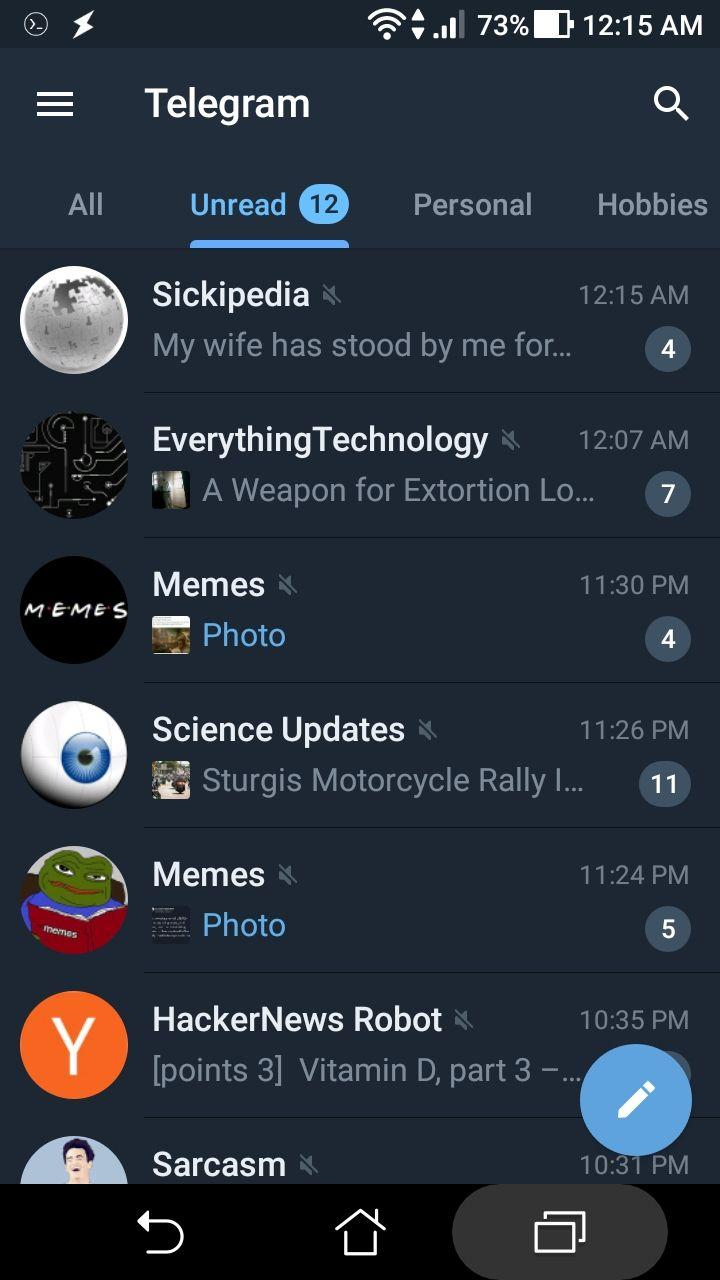
\includegraphics[height=0.9\textheight]{./logos/telegram-front}
			\end{center}
	\end{frame}
	
	\frontpic{Telegram for Desktop}{telegram-2nd}
	
	\frontpic{Telegram for Web}{telegram-web}
	
	\begin{frame}
		\frametitle{Advantages of Telegram}
		\begin{multicols}{2}
		\begin{itemize}
			\item<1-> 2GB file size limit
			\item<2-> Platform independent 
			\item<3-> Supports and compiles LaTeX.
			\item<4-> Can create quizzes and polls.
			\item<5-> Tabs for organization.
			\item<6-> Secure
			\item<6-> Pinned messages
		\end{itemize}		
	\end{multicols}
	\end{frame}

    \section{FOSS for Test Correction}
    \begin{frame}
    	\frametitle{FOSS for Teachers}
    	\begin{center}
    		\textbf{\LARGE FOSS for Test Correction}
    	\end{center} 
    \end{frame}
	
	\frontpic{Exam Auto-Checker}{autochecker}
	
	\begin{frame}
		\frametitle{Rationale}
		\begin{itemize}
			\item<1-> 
			Converting worksheets to Google Forms is tedious.
			\item<2-> 
			Manual checking and recording of student outputs is time-consuming.
		\end{itemize}		
	\end{frame}

    \begin{frame}
    	\frametitle{Strengths}
    	\begin{itemize}
    		\item<1-> 
    		Can be used with any chat app.
    		\item<2-> 
    		Automatically checks, saves, and records student outputs.
    		\item<3-> 
    		Multi-platform --- can be used in Windows, Linux, and Android.
    		\item<4-> 
    		Can check most types of test: Multiple choice, True/False, Matching type, Fill in the blank.
    		\item<5-> 
    		Does not consume data.
    	\end{itemize}		
    \end{frame}

    \begin{frame}
    	\frametitle{Weaknesses}
    	\begin{itemize}
    		\item<1-> 
    		Cannot check Math solutions.
    		\item<2-> 
    		Accuracy depends on input.
     	\end{itemize}		
    \end{frame}

    \begin{frame}
    	\begin{center}
    		\textbf{\LARGE Usage}
    	\end{center}		
    \end{frame}

    \frontpic{Create answer key.}{ans-key}
    
    \frontpic{Send worksheet.}{send-worksheet}
    
    \frontpic{Copy student's input.}{copy-input}
    
    \frontpic{Paste input to app.}{paste-to-app}
    
    \frontpic{Enter assessment type.}{type-assessment}
	
	\frontpic{Browse to output folder.}{browse-folder}
	
	\frontpic{Browse to answer key.}{browse-ans-key}
	
	\frontpic{Click Submit.}{submit}
	
	\frontpic{Click Save.}{save}
	
	\frontpic{The result.}{output-folder}
	
	\frontpic{The recorded scores.}{record}
	
    \begin{frame}
    	\begin{center}
    		If interested, please visit
    		
    		\vspace*{1em}
    		
    		\footnotesize{https://github.com/cityofsmiles/ExamAutoChecker}
    	\end{center}
    \end{frame}

    \begin{frame}
    	\begin{center}
    		\textbf{\LARGE Thank you!}
    	\end{center}
    \end{frame}

	\begin{frame}
		\frametitle{Online Sources}
		\tiny 
		https://mb.com.ph/2020/08/19/case-against-facebook-use-in-education/
\newline
		
		https://www.gmanetwork.com/news/money/companies/753042/microsoft-s-software-alliance-says-64-of-companies-in-philippines-use-unlicensed-software/story/
\newline
		
		https://cnnphilippines.com/news/2020/8/4/PhilHealth-Ricardo-Morales-overpriced-IT-projects-corruption.html?fbclid=IwAR2t9HjNjCuzeXZWpIexCmBoJjzjA0sn2ubjnefsxj01uT-sYiY4WppUkuQ
\newline
		
		https://www.androidheadlines.com/2020/07/google-misled-users-over-privacy-issues-according-to-regulator.html
\newline
		
		https://www.cnet.com/news/google-alphabet-earnings-fourth-quarter-2018/
\newline
		
		https://businessmirror.com.ph/2020/09/04/the-advantages-of-using-linux/
\newline


    https://www.tomsguide.com/news/chrome-google-site-data-special-treatment \newline

    https://arstechnica.com/information-technology/2020/10/study-shows-which-messengers-leak-your-data-drain-your-battery-and-more/
		
	\end{frame}	
	
		\begin{frame}
			\frametitle{Online Sources}
			\tiny 
			 
			https://securityboulevard.com/2020/08/phishing-campaign-uses-internal-email-to-trick-employees-into-sharing-office-365-credentials/
\newline
			
			https://www.channelasia.tech/article/679771/supreme-court-philippines-rolls-microsoft-365-unveils-virtual-courtrooms/
\newline
			
			https://healthitsecurity.com/news/bec-phishing-campaigns-bypass-mfa-target-office-365-executive-accounts \newline
			
			https://sea.pcmag.com/encryption-products/38803/windows-computers-account-for-83-of-all-malware-attacks-in-q1-2020 \newline
			
			https://www.bleepingcomputer.com/news/microsoft/windows-10-themes-can-be-abused-to-steal-windows-passwords/ \newline
			
			https://www.zdnet.com/article/malware-gang-uses-net-library-to-generate-excel-docs-that-bypass-security-checks/ \newline
			
			https://itsfoss.com/linux-runs-top-supercomputers/ \newline
			
			https://www.gnu.org/education/edu-schools.html \newline
			
			https://www.euroweeklynews.com/2020/10/10/google-provide-police-with-your-keyword-searches/amp/
		\end{frame}	
	
\end{document}